% Rebuild: mkdir -p build
% pdflatex -interaction=nonstopmode -halt-on-error -output-directory=build HKT_substitutes_derivation.tex
% Repeat the pdflatex command to resolve equation references.
% Recompute the illustrative figure and checks: python3 verify_derivation.py
\documentclass[11pt,a4paper]{article}
\usepackage[margin=25mm]{geometry}
\usepackage[T1]{fontenc}
\usepackage{lmodern,microtype}
\usepackage{amsmath,amssymb,amsthm,mathtools}
\usepackage{booktabs,tabularx,array,graphicx,float}
\usepackage[dvipsnames]{xcolor}
\usepackage[colorlinks=true,linkcolor=MidnightBlue,urlcolor=MidnightBlue,citecolor=MidnightBlue]{hyperref}
\usepackage{enumitem}
\setlist{nosep}
\setlength{\parskip}{5pt}
\setlength{\parindent}{0pt}
\setlength{\emergencystretch}{2em}
\newtheorem{proposition}{Proposition}
\newtheorem{corollary}{Corollary}
\newtheorem{remark}{Remark}
\newcommand{\E}{\mathbb E}
\newcommand{\asym}{\sim}
\newcommand{\HKT}{\textnormal{HKT}}
\title{The Single-Country HKT Model with\\
\texorpdfstring{$\xi_u<\lambda_u$ and $0<\rho<1$}{xi-u < lambda-u and 0 < rho < 1}}
\author{Derivation and verification note}
\date{17 November 2026}

\begin{document}
\maketitle
\begin{abstract}
The proposed restrictions select the substitutes branch of the model in Hirano,
Kishi, and Toda (16 August 2026). They satisfy the paper's existing condition
$\kappa=(\xi_u-\lambda_u)(\rho-1)>0$. With active initial innovation,
$\lambda_u>\lambda_b=\xi_b$, and relative risk aversion $\gamma<1$, the unique
equilibrium continues to exhibit a bubble throughout state $u$ and no bubble in
the absorbing state $b$. We derive the exact equilibrium, conditional asymptotic
rates, the infinite-product bubble characterization, and implications for factor
shares and wages. The economic interpretation changes: unskilled-labor-augmenting
productivity grows faster, and substitutability allows its effective input to
dominate final production. The equilibrium skill premium declines, even though
capturing more bubble value in IPO proceeds raises it in the paper's separate
partial-equilibrium experiment. A rising price-dividend ratio need not imply a
rising per-share price.
\end{abstract}

\section{Source, notation, and maintained assumptions}
The source is the user-supplied PDF of \emph{General-Purpose Technologies and
Stock Market Bubbles}, dated 16 August 2026, CIGS Working Paper 26-013E.
The corresponding publisher copy is available
\href{https://cigs.canon/en/uploads/2026/08/WP26-013E_260816_hirano.pdf}{here}.
The local PDF has 60 pages; its first page is a cover, so printed page $p$ is
PDF page $p+1$. This note reconstructs the relevant model equations and supplies
a derivation; it is not a transcription of the entire paper.

\textbf{Notation clarification.} The knowledge spillover exponent written as
\emph{zeta} in the request is denoted by $\xi_z$ in HKT. HKT uses
$\zeta_t=A_{Xt}H/(A_{Lt}L)$ for a different object, relative effective
productivity. Here we use $\xi_u$ for the requested exponent. Also,
$1/\rho$ is the elasticity of substitution \emph{in production}, whereas
$\gamma$ is relative risk aversion. Thus $0<\rho<1$ means substitution elasticity
above one and does not impose $\gamma<1$.

The baseline maintained restrictions are
\begin{gather}
0<\alpha,\beta<1,\quad \sigma>1,\quad a,H,L,A_X,A_L>0,
\quad 0<\pi<1,\quad \gamma\geq0,\label{eq:primitives}\\
0\leq\xi_u<\lambda_u,\qquad 0<\rho<1,\qquad
0\leq\lambda_b=\xi_b<\lambda_u.\label{eq:assumptions}
\end{gather}
The state process satisfies $\Pr(z_{t+1}=u\mid z_t=u)=\pi$ and
$\Pr(z_{t+1}=b\mid z_t=b)=1$. Preferences are the original two-period
Epstein--Zin specification with unit EIS:
\begin{equation}
U_t=(1-\beta)\log c^y_t+
\frac{\beta}{1-\gamma}\log\E_t[(c^o_{t+1})^{1-\gamma}],\label{eq:utility}
\end{equation}
with the expected-log limit at $\gamma=1$. We impose $\gamma<1$ only for the
bubble theorem below. All asymptotic statements in state $u$ are conditional
on that state continuing. The transition occurs in finite time almost surely
when $\pi\in(0,1)$.

Define the positive constants
\begin{align}
\kappa&=(\xi_u-\lambda_u)(\rho-1)
       =(\lambda_u-\xi_u)(1-\rho)>0,\label{eq:kappa}\\
r&=\frac{\kappa}{\rho}
  =(\lambda_u-\xi_u)\left(\frac1\rho-1\right)>0,\label{eq:r}\\
K&=\frac{\beta\sigma(1-\alpha)}{(\sigma-1)\alpha}
       \left(\frac{A_XH}{A_LL}\right)^{\rho-1},\qquad
c_* = \frac1{aH}+1-\beta.\label{eq:constants}
\end{align}
HKT's Assumption 6, printed p.~21, already permits this branch. Its main
discussion emphasizes the alternative branch $\xi_u>\lambda_u,\rho>1$.

\section{Reconstructing the exact equilibrium}
\subsection{Production, prices, and asset supply}
Let $\phi_t\in(0,1]$ be the share of skilled workers producing intermediate
goods. The remaining share $1-\phi_t$ conducts R\&D. The normalized variety
aggregator in HKT implies $X_t=H\phi_t$ under symmetry. Write
\begin{align}
A_{Xt}&=A_X n_t^{\xi_{z_t}}, & A_{Lt}&=A_L n_t^{\lambda_{z_t}},\label{eq:productivities}\\
Y_t&=\left[\alpha(A_Xn_t^{\xi_{z_t}}H\phi_t)^{1-\rho}
 +(1-\alpha)(A_Ln_t^{\lambda_{z_t}}L)^{1-\rho}\right]^{1/(1-\rho)}.
\label{eq:output}
\end{align}
With $F_X=\alpha F^\rho X^{-\rho}$ and
$F_L=(1-\alpha)F^\rho L^{-\rho}$, the equilibrium wages are
\begin{align}
w_{Ht}&=\frac{\sigma-1}{\sigma}\alpha Y_t^\rho
             (A_Xn_t^{\xi_{z_t}})^{1-\rho}(H\phi_t)^{-\rho},\label{eq:wH}\\
w_{Lt}&=(1-\alpha)Y_t^\rho
             (A_Ln_t^{\lambda_{z_t}})^{1-\rho}L^{-\rho}.\label{eq:wL}
\end{align}
One share is issued by each firm. Throughout this note $Q_t$ and $D_t$ are
the \emph{per-share} ex-dividend price and dividend, respectively:
\begin{align}
D_t&=\frac{w_{Ht}H\phi_t}{(\sigma-1)n_t},\label{eq:dividend}\\
n_{t+1}&=[1+aH(1-\phi_t)]n_t.\label{eq:knowledge}
\end{align}
The young buy both incumbent shares and newly issued shares, so the stock-market
clearing equation uses $n_{t+1}$:
\begin{equation}
n_{t+1}Q_t=\beta(Hw_{Ht}+Lw_{Lt}).\label{eq:stockclear}
\end{equation}
Occupational optimality requires
\begin{equation}
an_tQ_t\leq w_{Ht},\qquad
(1-\phi_t)(w_{Ht}-an_tQ_t)=0.\label{eq:occupation}
\end{equation}
Thus active innovation implies $Q_t=w_{Ht}/(an_t)$. If innovation is inactive,
$\phi_t=1$, $n_{t+1}=n_t$, and instead
$Q_t=\beta(Hw_{Ht}+Lw_{Lt})/n_t$.

\subsection{Labor allocation and the initial innovation condition}
Under active innovation, substitute $Q_t=w_{Ht}/(an_t)$ into
\eqref{eq:stockclear} and divide by $Hw_{Ht}$. This gives
\begin{equation}
\frac1{aH}+1-\phi_t=\beta+\beta\frac{Lw_{Lt}}{Hw_{Ht}}.\label{eq:clearingratio}
\end{equation}
From \eqref{eq:wH}--\eqref{eq:wL},
\begin{equation}
\beta\frac{Lw_{Lt}}{Hw_{Ht}}
 =K n_t^{(\xi_{z_t}-\lambda_{z_t})(\rho-1)}\phi_t^\rho.
\end{equation}
Consequently the exact state-$u$ equilibrium is characterized by
\begin{equation}
\boxed{\phi_t+K n_t^\kappa\phi_t^\rho=c_*.}\label{eq:allocation}
\end{equation}
The left side is continuous and strictly increasing in $\phi_t>0$. A unique
interior solution exists precisely when
\begin{equation}
\boxed{\beta+K n_t^\kappa>\frac1{aH}.}\label{eq:innovation}
\end{equation}
We maintain this strict inequality at $n_0$; it is HKT equation (4.4).
If $\beta<1/(aH)$, it is equivalent to
\begin{equation}
n_0>\left[\frac{1/(aH)-\beta}{K}\right]^{1/\kappa}.
\end{equation}
If $\beta\geq1/(aH)$, every $n_0>0$ satisfies it. If it fails, the equilibrium
in state $u$ has $\phi_t=1$ and $n_t=n_0$ until the regime changes. Knowledge
does not grow spontaneously past the threshold. The growing-path bubble result
therefore cannot be inferred from the two new inequalities alone.

\section{Innovation and conditional growth}
\begin{proposition}[Labor reallocation and its exact rate]
Under \eqref{eq:primitives}--\eqref{eq:assumptions} and initial active innovation,
the state-$u$ path satisfies
\begin{gather}
\phi_t\downarrow0,\qquad
\frac{n_{t+1}}{n_t}\uparrow G_u:=1+aH,\label{eq:growth}\\
\phi_t\asym C_\phi n_t^{-r},\qquad
C_\phi=\left(\frac{c_*}{K}\right)^{1/\rho},\qquad
\frac{n_t}{G_u^t}\longrightarrow\bar n\in(0,\infty).\label{eq:phiasym}
\end{gather}
Here $x_t\asym C y_t$ means $x_t/(Cy_t)\to1$.
\end{proposition}
\begin{proof}
For fixed $\phi>0$, the left side of \eqref{eq:allocation} increases in $n$.
Hence $\phi(n)$ decreases as knowledge accumulates. Since innovation is active
initially, $n_{t+1}/n_t\geq g_0:=1+aH(1-\phi_0)>1$; innovation remains active
and $n_t\to\infty$. Equation \eqref{eq:allocation} then implies $\phi_t\to0$.
Moreover,
\begin{equation}
Kn_t^\kappa\phi_t^\rho=c_*-\phi_t\longrightarrow c_*,
\end{equation}
which proves the equivalent in \eqref{eq:phiasym} and gives the global bound
$\phi_t\leq C_\phi n_t^{-r}\leq C_\phi n_0^{-r}g_0^{-rt}$. Thus
$\sum_t\phi_t<\infty$. Finally,
\begin{equation}
\frac{n_t}{G_u^t}
=n_0\prod_{s=0}^{t-1}\left(1-\frac{aH}{G_u}\phi_s\right)
\end{equation}
has a strictly positive finite limit because the subtracted terms are summable
and each factor is positive.
\end{proof}
Implicit differentiation also provides the exact elasticity
\begin{equation}
\boxed{\frac{d\log\phi}{d\log n}
=-\frac{\kappa(c_*-\phi)}{\rho c_*+(1-\rho)\phi}
\longrightarrow-r.}\label{eq:elasticity}
\end{equation}
Therefore $1-\phi_t\uparrow1$: almost all skilled workers eventually conduct
R\&D, conditional on state $u$ continuing. For a fixed spillover gap
$\lambda_u-\xi_u$, a lower $\rho$ raises the \emph{asymptotic exponent} $r$.
This does not order entire transition paths across different parameterizations,
because $K$ and initial allocations change as well.

\section{What changes economically: production, wages, and dividends}
Define the relative effective input
\begin{equation}
v_t=\frac{A_Xn_t^{\xi_u}H\phi_t}{A_Ln_t^{\lambda_u}L}.
\end{equation}
By \eqref{eq:phiasym},
\begin{equation}
v_t\asym\frac{A_XH}{A_LL}C_\phi
 n_t^{\xi_u-\lambda_u-r}
=\frac{A_XH}{A_LL}C_\phi n_t^{-(\lambda_u-\xi_u)/\rho}
\longrightarrow0.\label{eq:effectiveinput}
\end{equation}
Since $1-\rho>0$, factorizing output gives
\begin{equation}
Y_{ut}=A_LL n_t^{\lambda_u}
 \left[\alpha v_t^{1-\rho}+1-\alpha\right]^{1/(1-\rho)}
\asym C_Y n_t^{\lambda_u},\qquad
C_Y=(1-\alpha)^{1/(1-\rho)}A_LL.\label{eq:Yasym}
\end{equation}
Thus the unskilled effective input dominates the CES aggregate. This is
consistent with $1/\rho>1$: the relatively scarce knowledge-intensive input
does not become a binding aggregate production bottleneck.

\subsection{The skill premium has a simple exact formula}
Rearrange \eqref{eq:clearingratio} to obtain
\begin{equation}
\boxed{\frac{w_{Ht}}{w_{Lt}}
=\frac{\beta L}{H(c_*-\phi_t)}
\downarrow\frac{\beta L}{Hc_*}>0.}\label{eq:premium}
\end{equation}
The premium declines along the state-$u$ equilibrium path. The limit need not
exceed one: the labels ``skilled'' and ``unskilled'' identify technologies and
occupations, not an imposed ranking of equilibrium wages. At the same time,
both wage levels have the same leading growth rate:
\begin{equation}
w_{Lt}\asym\frac{C_Y}{L}n_t^{\lambda_u},\qquad
w_{Ht}\asym\frac{\beta C_Y}{Hc_*}n_t^{\lambda_u}.\label{eq:wageasym}
\end{equation}
The skilled wage keeps pace despite its lower productivity exponent because
skilled labor remaining in current production becomes scarce.

\subsection{Prices, dividends, and market capitalization}
Combining the wage equivalents with occupational indifference and
\eqref{eq:dividend},
\begin{align}
Q_{ut}&\asym C_Q n_t^{\lambda_u-1}, &
C_Q&=\frac{\beta C_Y}{aHc_*},\label{eq:Qasym}\\
D_{ut}&\asym C_D n_t^{\lambda_u-1-r}, &
C_D&=\frac{\beta C_Y C_\phi}{c_*(\sigma-1)}.\label{eq:Dasym}
\end{align}
The dividend yield and its inverse satisfy
\begin{equation}
\boxed{\frac{D_{ut}}{Q_{ut}}=\frac{aH}{\sigma-1}\phi_t
\asym\frac{aH C_\phi}{\sigma-1}n_t^{-r},\qquad
\frac{Q_{ut}}{D_{ut}}\asym\frac{\sigma-1}{aH C_\phi}n_t^r.}
\label{eq:yield}
\end{equation}
In particular, the limiting gross growth factor of $Q/D$ is
\begin{equation}
\boxed{G_{Q/D}=G_u^{(\lambda_u-\xi_u)(1-\rho)/\rho}>1.}\label{eq:PDgrowth}
\end{equation}

\begin{table}[htbp]
\centering
\caption{Conditional state-$u$ asymptotic rates. All constants are positive.}
\begin{tabular}{lll}
\toprule
Object & Order in $n_t$ & Limiting gross growth factor\\
\midrule
Production employment share $\phi_t$ & $n_t^{-r}$ & $G_u^{-r}$\\
Output $Y_t$, wages $w_{Ht},w_{Lt}$ & $n_t^{\lambda_u}$ & $G_u^{\lambda_u}$\\
Per-share price $Q_t$ & $n_t^{\lambda_u-1}$ & $G_u^{\lambda_u-1}$\\
Per-share dividend $D_t$ & $n_t^{\lambda_u-1-r}$ & $G_u^{\lambda_u-1-r}$\\
Price-dividend ratio $Q_t/D_t$ & $n_t^r$ & $G_u^r$\\
Incumbent capitalization $n_tQ_t$ & $n_t^{\lambda_u}$ & $G_u^{\lambda_u}$\\
Aggregate dividends $n_tD_t$ & $n_t^{\lambda_u-r}$ & $G_u^{\lambda_u-r}$\\
\bottomrule
\end{tabular}
\end{table}

A bubble does not require an increasing per-share price. If $\lambda_u<1$,
$Q_t\to0$ along the continuing-$u$ path; if $\lambda_u=1$, it converges to
$C_Q$; if $\lambda_u>1$, it diverges. In all cases $Q_t/D_t\to\infty$.
Aggregate dividends may also increase or decrease, depending on the sign of
$\lambda_u-r$. Two useful ratios are
\begin{equation}
\frac{n_tQ_t}{Y_t}\longrightarrow
\frac{\beta}{1+aH(1-\beta)}>0,
\qquad
\frac{n_tD_t}{Y_t}\asym\frac{\beta}{c_*(\sigma-1)}\phi_t\longrightarrow0.
\label{eq:aggregateratios}
\end{equation}
Here $n_tQ_t$ values incumbent firms after current dividends. The end-of-date
portfolio includes new issues and is worth $n_{t+1}Q_t$; its output ratio has
the same limit multiplied by $G_u$.

\subsection{Factor shares and the interpretation of the two branches}
The final-good revenue share accruing to purchases of the knowledge-intensive
input is
\begin{equation}
s_{Xt}=\frac{P_tX_t}{Y_t}
=\frac{\alpha v_t^{1-\rho}}{\alpha v_t^{1-\rho}+1-\alpha}\longrightarrow0,
\qquad
\frac{Lw_{Lt}}{Y_t}=1-s_{Xt}\longrightarrow1.\label{eq:shares}
\end{equation}
The skilled wage bill \emph{in current production} is
$H\phi_t w_{Ht}/Y_t=(\sigma-1)s_{Xt}/\sigma$, and aggregate profits are
$n_tD_t/Y_t=s_{Xt}/\sigma$. Both vanish as output shares. This does not mean
the income of all skilled workers vanishes: their R\&D income is financed by
IPO proceeds, and $Hw_{Ht}/Y_t\to\beta/c_*$.

\begin{table}[htbp]
\centering\small
\caption{The mathematical condition is shared; the technology story differs.}
\begin{tabularx}{\textwidth}{@{}l>{\raggedright\arraybackslash}X>{\raggedright\arraybackslash}X@{}}
\toprule
 & HKT's emphasized branch & Branch in this note\\
\midrule
Spillover ordering & $\xi_u>\lambda_u$ & $\xi_u<\lambda_u$\\
Substitution elasticity & $1/\rho<1$ & $1/\rho>1$\\
Relative effective input & $v_t\to\infty$ & $v_t\to0$\\
Why the $L$ term dominates & Complementarity: the relatively scarce $L$ input limits production & Substitutability: the rapidly expanding $L$ input dominates production\\
Common dynamics & \multicolumn{2}{l}{$\kappa>0$, $\phi_t\to0$, $Y_t\asym C_Yn_t^{\lambda_u}$, $Q_t/D_t\to\infty$}\\
\bottomrule
\end{tabularx}
\end{table}

\section{The asset-pricing proof}
\subsection{The balanced state is fundamental}
Let $\phi_b$ be the unique interior root of
\begin{equation}
\phi_b+K\phi_b^\rho=c_*\label{eq:phib}
\end{equation}
when $\beta+K>1/(aH)$. Otherwise set $\phi_b=1$; the equality case is also
the no-innovation boundary. Define
\begin{equation}
G_b=1+aH(1-\phi_b)<G_u.
\end{equation}
Since both productivities have exponent $\lambda_b$, output and both wages
scale exactly as $n_t^{\lambda_b}$. Prices and dividends scale as
$n_t^{\lambda_b-1}$, whether or not innovation continues. Their ratio is
constant and positive. More explicitly, with $y_b=D_{bt}/Q_{bt}$,
\begin{equation}
y_b=\begin{cases}
\displaystyle\frac{aH}{\sigma-1}\phi_b,&\phi_b<1,\\[4pt]
\displaystyle\frac{1}{\beta(\sigma-1)}
\frac{H\bar w_{Hb}}{H\bar w_{Hb}+L\bar w_{Lb}},&\phi_b=1,
\end{cases}\label{eq:yieldb}
\end{equation}
where $w_{ib}(n)=\bar w_{ib}n^{\lambda_b}$. At the entry boundary the two
formulas agree.

With no remaining uncertainty, $m_{t,t+1}=Q_t/(Q_{t+1}+D_{t+1})$, hence
\begin{equation}
m_{t,T}Q_T=Q_t(1+y_b)^{-(T-t)}\longrightarrow0.
\end{equation}
Therefore $Q_t=V_t$ in state $b$, where
$V_t=\E_t\sum_{s>t}m_{t,s}D_s$.

\subsection{The exact two-series test}
Substituting the consumption and portfolio rules into the Epstein--Zin SDF
cancels type-specific wages and yields
\begin{equation}
m_{t,t+1}=\frac{Q_t(Q_{t+1}+D_{t+1})^{-\gamma}}
 {\E_t[(Q_{t+1}+D_{t+1})^{1-\gamma}]}.\label{eq:sdf}
\end{equation}
For each date $s$ on the history that remained in $u$ through $s-1$, let
$\Pi_{zs}=Q_{zs}+D_{zs}$, $z\in\{u,b\}$. These are the two possible
payoffs at the \emph{same predetermined knowledge stock} $n_s$.
Define
\begin{equation}
a_s=\frac{D_{us}}{Q_{us}}+
\frac{1-\pi}{\pi}\left(1+\frac{D_{us}}{Q_{us}}\right)
\left(\frac{\Pi_{bs}}{\Pi_{us}}\right)^{1-\gamma}.\label{eq:as}
\end{equation}
Direct multiplication of the continuing-state discount factors gives
\begin{equation}
\pi^{T-t}m^{u}_{t,T}Q_{uT}
=Q_{ut}\prod_{s=t+1}^{T}(1+a_s)^{-1}.\label{eq:product}
\end{equation}
The contribution of already-transitioned histories to the expected discounted
terminal price vanishes: each such history is subsequently fundamental, and
its entry-date discounted price is bounded by a summable collection of
nonnegative state-price contributions. This is the dominated-convergence
argument in HKT Proposition 2.3 and Appendix A.2. Consequently
\begin{equation}
\boxed{\frac{B_{ut}}{Q_{ut}}=
\prod_{s=t+1}^{\infty}(1+a_s)^{-1},\qquad B_t:=Q_t-V_t.}\label{eq:bubblefraction}
\end{equation}
For nonnegative $a_s$, this product is positive if and only if
$\sum_s a_s<\infty$. Equivalently,
\begin{equation}
\boxed{B_{ut}>0\quad\Longleftrightarrow\quad
\sum_{s>t}\frac{D_{us}}{Q_{us}}<\infty
\quad\text{and}\quad
\sum_{s>t}\left(\frac{\Pi_{bs}}{\Pi_{us}}\right)^{1-\gamma}<\infty.}
\label{eq:two-series}
\end{equation}
The first series alone does not suffice in a model with anticipated complete
collapse.

\subsection{Evaluation under the proposed restrictions}
Equation \eqref{eq:yield} and geometric knowledge growth imply
\begin{equation}
\frac{D_{ut}}{Q_{ut}}\asym C_y n_t^{-r},\qquad
\sum_t\frac{D_{ut}}{Q_{ut}}<\infty.\label{eq:firstsum}
\end{equation}
In state $b$, $Q_{bt}=\bar Q_b n_t^{\lambda_b-1}$ with $\bar Q_b>0$,
including at the no-innovation corner. Since $y_b>0$ is constant and the
state-$u$ yield vanishes,
\begin{equation}
\frac{\Pi_{bt}}{\Pi_{ut}}
\asym C_\Pi n_t^{\lambda_b-\lambda_u},\qquad C_\Pi>0.\label{eq:payoffratio}
\end{equation}
Thus, when $\lambda_u>\lambda_b$ and $\gamma<1$,
\begin{equation}
\left(\frac{\Pi_{bt}}{\Pi_{ut}}\right)^{1-\gamma}
\asym C_\Pi^{1-\gamma}n_t^{-\delta},\qquad
\delta=(\lambda_u-\lambda_b)(1-\gamma)>0,\label{eq:secondsum}
\end{equation}
which is also summable.

\begin{proposition}[The bubble survives the proposed change]
Maintain \eqref{eq:primitives}--\eqref{eq:assumptions}, initial active innovation,
and $\gamma<1$. The unique equilibrium has $Q_t>V_t$ at every state-$u$
history, an exponentially increasing conditional price-dividend ratio, and
$Q_t=V_t$ with constant $Q_t/D_t$ in state $b$.
\end{proposition}
\begin{proof}
The equilibrium is uniquely pinned down by \eqref{eq:allocation}, or the
no-innovation corner, together with \eqref{eq:knowledge} and the price
formulas. Both series in \eqref{eq:two-series} converge by
\eqref{eq:firstsum}--\eqref{eq:secondsum}. The state-$b$ argument was proved
above. These arguments apply to the tail following every state-$u$ history.
\end{proof}

\begin{corollary}[Bubble fraction]
Along a continuing-$u$ history, $B_{ut}/Q_{ut}\uparrow1$. More precisely,
\begin{equation}
\frac{V_{ut}}{Q_{ut}}=O\!\left(n_t^{-r}+n_t^{-\delta}\right).
\end{equation}
\end{corollary}
\begin{proof}
The tail of a convergent nonnegative series vanishes, so the tail product in
\eqref{eq:bubblefraction} increases to one. Also
$0\leq1-\prod_{s>t}(1+a_s)^{-1}\leq\sum_{s>t}a_s$.
Equations \eqref{eq:firstsum}--\eqref{eq:secondsum} and a uniform geometric
lower bound on future knowledge growth give the stated order.
\end{proof}
For every fixed $\pi\in(0,1)$, its value only rescales the second term in
\eqref{eq:as}, so it does not change convergence or bubble existence. It
\emph{does} change the bubble fraction: for a fixed technology path, a higher
$\pi$ raises that fraction. It also changes expected remaining duration,
$1/(1-\pi)$. The restrictions $\pi>0$ and $\pi<1$ should not be replaced by
endpoint values without redoing the argument.

\paragraph{If other assumptions are not retained.}
Keep $\kappa>0$, initial active innovation, the unit-EIS model, and
$\xi_b=\lambda_b$, but allow either ordering of $\lambda_b$ and $\lambda_u$.
The same derivation gives the exact criterion
\begin{equation}
\boxed{B_{ut}>0\quad\Longleftrightarrow\quad
(\lambda_u-\lambda_b)(1-\gamma)>0.}\label{eq:generalcriterion}
\end{equation}
At equality the second series diverges; if the product is negative its terms
grow rather than vanish. In the intended collapse-to-a-lower-payoff regime,
$\lambda_b<\lambda_u$, this reduces to $\gamma<1$. Hence $\rho<1$ cannot
replace the separate risk-aversion restriction. Mathematically, the reverse
ordering $\lambda_b>\lambda_u$ can satisfy the criterion when $\gamma>1$;
that is a different transition interpretation from HKT's maintained assumptions.
If initial innovation is inactive, $n_t$ is constant in state $u$ and its
strictly positive dividend yield is constant, so already the first series
diverges and there is no state-$u$ bubble.

\section{Regime transition and the productive legacy}
At the same inherited knowledge stock, the exact comparison is
\begin{equation}
\frac{Y_b(n)}{Y_u(n)}
=n^{\lambda_b-\lambda_u}
\frac{F(A_XH\phi_b,A_LL)}{F(A_XHn^{\xi_u-\lambda_u}\phi_u(n),A_LL)}.
\end{equation}
Together with \eqref{eq:Yasym} and \eqref{eq:Qasym}, this implies
\begin{equation}
\frac{Y_{bt}}{Y_{ut}}\asym C_{Yu,b}n_t^{\lambda_b-\lambda_u}\to0,
\qquad
\frac{Q_{bt}}{Q_{ut}}\asym C_{Qu,b}n_t^{\lambda_b-\lambda_u}\to0.
\end{equation}
Because $n_t/n_{t-1}\to G_u$, the actual across-date comparisons have the
same power:
\begin{equation}
\boxed{\frac{Y_{bt}}{Y_{u,t-1}}\asym\widetilde C_Y n_t^{\lambda_b-\lambda_u}\to0,
\qquad
\frac{Q_{bt}}{Q_{u,t-1}}\asym\widetilde C_Q n_t^{\lambda_b-\lambda_u}\to0.}
\label{eq:crash}
\end{equation}
The constants are generally different. These are statements about a
\emph{sufficiently late} transition. They do not prove an output or price decline
at every possible finite transition date, or identify the pure causal effect of
removing the bubble while holding technology fixed.

The limits $\phi_u\to0<\phi_b$ imply that a sufficiently late transition raises
the production share and reduces R\&D and knowledge growth. There is a useful
finite-date qualification. If $b$ also has active innovation, comparing
\eqref{eq:allocation} and \eqref{eq:phib} gives
\begin{equation}
\phi_u(n)<\phi_b\quad\Longleftrightarrow\quad n>1.
\end{equation}
Thus $n_0\geq1$ guarantees the usual direction at any subsequent transition.
For $n<1$, the direction can reverse. If $\phi_b=1$, any transition from an
innovating $u$ state reduces R\&D. The threshold $n=1$ uses the paper's common
productivity intercepts and chosen units for knowledge.

Let $\tau$ be the transition date. For every fixed $k\geq0$,
\begin{align}
n_{\tau+k}&=G_b^k n_\tau,\\
Y_{\tau+k}&=\bar Y_b G_b^{k\lambda_b}n_\tau^{\lambda_b},\label{eq:legacy}\\
w_{i,\tau+k}&=\bar w_{ib}G_b^{k\lambda_b}n_\tau^{\lambda_b},\qquad i=H,L,
\end{align}
where $\bar Y_b=F(A_XH\phi_b,A_LL)$ and the wage constants follow from
the CES marginal products. Since $n_\tau$ increases with the duration of $u$,
a later transition strictly raises these levels at a fixed post-transition
horizon when $\lambda_b>0$. If $\lambda_b=0$, this level effect is zero.
The post-transition skill premium is independent of $\tau$ and $k$.

Under the new branch, $\lambda_b<\lambda_u$ does not imply
$\xi_b=\lambda_b<\xi_u$. For example, $\xi_u<\lambda_b<\lambda_u$ is allowed.
Thus describing the transition as a reduction in \emph{both} spillover
exponents requires the additional restriction $\lambda_b<\xi_u$. That extra
restriction is unnecessary for the bubble proof or \eqref{eq:crash}.

\section{Bubble-backed IPOs versus the equilibrium time path}
HKT Proposition 4.2 fixes $n_t,A_{Xt},A_{Lt},V_t,B_t$ and varies the fraction
$\chi\in[0,1]$ of bubble value captured in innovators' net IPO proceeds:
\begin{equation}
Q_t^{\mathrm{IPO}}(\chi)=V_t+\chi B_t.
\end{equation}
For an interior occupational choice,
$w_H(\phi(\chi))=an_t[V_t+\chi B_t]$. At fixed productivity,
\begin{equation}
\frac{d\log w_H}{d\log\phi}=-\rho(1-s_X)<0,
\qquad
\frac{d\log w_L}{d\log\phi}=\rho s_X>0,
\qquad
\frac{d\log(w_H/w_L)}{d\log\phi}=-\rho<0.
\end{equation}
Therefore the partial-equilibrium comparative statics remain valid for
$0<\rho<1$: a higher $\chi$ weakly reduces $\phi$, increases the skilled wage,
the skill premium, R\&D, and next-period knowledge, and reduces the unskilled
wage and current output. The changes are strict on the interior; a
no-innovation corner can produce a flat region.

This is compatible with \eqref{eq:premium}. In the partial-equilibrium
experiment, productivities and benchmark valuation components are fixed. Along
the actual time path they change with $n_t$, and $n_t^\kappa\phi_t^\rho$
increases to $c_*/K$, so the skill premium falls. The partial-equilibrium
experiment is not an alternative market-clearing equilibrium and cannot be
iterated with $V_t$ and $B_t$ held fixed.

\section{Boundary cases and the paper's extensions}
If $\rho=1$ or $\xi_u=\lambda_u$, then $\kappa=0$ and the interior allocation
and dividend yield are constant. The first series in \eqref{eq:two-series}
diverges. This reproduces HKT Proposition 4.4's knife-edge condition for a
constant price-dividend ratio. If $\xi_u<\lambda_u$ but $\rho>1$, then
$\kappa<0$: conditional on innovation, the production share rises with
knowledge, so it is a different case. The result here relies on changing the
signs together.

HKT's infinitely lived-cohort extension is also stated under $\kappa>0$ and
therefore already includes the present branch. With its own entry conditions
and admissible continuation-value solution, its allocation equation is
\begin{equation}
Kn_t^\kappa\phi_t^\rho+\eta\phi_t=M,
\quad \eta=1+\frac{\beta}{\sigma-1},\quad
M=(1-\beta)\left(1+\frac1{aH}\right).
\end{equation}
It gives $\phi_t\asym(M/K)^{1/\rho}n_t^{-r}$, so the growth powers and the
two bubble summability tests are unchanged. The two-period wage-premium
identity \eqref{eq:premium} should not be transferred to that extension:
its aggregate saving equation includes existing cohorts' financial wealth.

The main derivation retains unit EIS. HKT's Appendix B.2 studies non-unit EIS
for the endowment economy, where saving and equilibrium prices become
forward-looking. Its results do not by themselves justify substituting a
different EIS into the production allocation equation derived here.

\section{Illustrative verification and source correspondence}
The companion script \texttt{verify\_derivation.py} evaluates the original CES
marginal-product formulas independently of the simplified wage and yield
identities. It checks asset clearing with $n_{t+1}$ shares, factor-payment
accounting, the implicit derivative, asymptotic coefficients, the state-price
product, and innovation corners. A 30-case grid covers both signs of the
spillover gap and both sides of $\rho=1$ (excluding the singular CES formula
at $\rho=1$). Full results and the source SHA-256 are in
\texttt{verification.json}.

The illustration uses
\begin{gather*}
\alpha=\beta=\rho=\tfrac12,\quad \sigma=2,\quad a=0.2,\quad H=L=1,\\
A_X=0.01,\quad A_L=1,\quad n_0=1,\quad
\xi_u=0.2,\quad\lambda_u=0.7,\quad\lambda_b=\xi_b=0.1,\\
\pi=0.95,\qquad\gamma=0.5.
\end{gather*}
Here $K=10$, $c_*=5.5$, $\kappa=0.25$, $r=0.5$, and $G_u=1.2$.
These are illustrative parameters, not calibration estimates or empirical
evidence. The conditional price-dividend ratio grows asymptotically by
$1.2^{0.5}$ per period, while the per-share price changes by $1.2^{-0.3}$.

The bubble fractions use the exact finite product through $T=800$. To control
its infinite tail, let $C_y=aHC_\phi/(\sigma-1)$,
$\Pi_b(n)=\bar\Pi_b n^{\lambda_b-1}$, and $C_R=\bar\Pi_b/C_Q$.
The CES lower bound $Y_u(n)\geq C_Yn^{\lambda_u}$ implies
$Q_u(n)\geq C_Qn^{\lambda_u-1}$, and hence
$\Pi_b/\Pi_u\leq C_Rn^{-(\lambda_u-\lambda_b)}$.
For $g_T=1+aH(1-\phi_T)>1$, future knowledge is at least $n_Tg_T^j$, so
\begin{align}
\sum_{s>T}\log(1+a_s)&\leq\sum_{s>T}a_s\leq\varepsilon_T,\\
\varepsilon_T&=
\frac{C_y n_T^{-r}}{g_T^r-1}
+\frac{1-\pi}{\pi}(1+C_y n_T^{-r})
\frac{C_R^{1-\gamma}n_T^{-\delta}}{g_T^\delta-1}.
\end{align}
If $b_t^{(T)}=\prod_{s=t+1}^T(1+a_s)^{-1}$, then for $t\leq T$,
\begin{equation}
b_t^{(T)}e^{-\varepsilon_T}\leq B_{ut}/Q_{ut}\leq b_t^{(T)}.
\end{equation}
The script verifies $\varepsilon_{800}<10^{-16}$ in this illustration.
This bound controls truncation; ordinary floating-point rounding remains.

\begin{figure}[p]
\centering
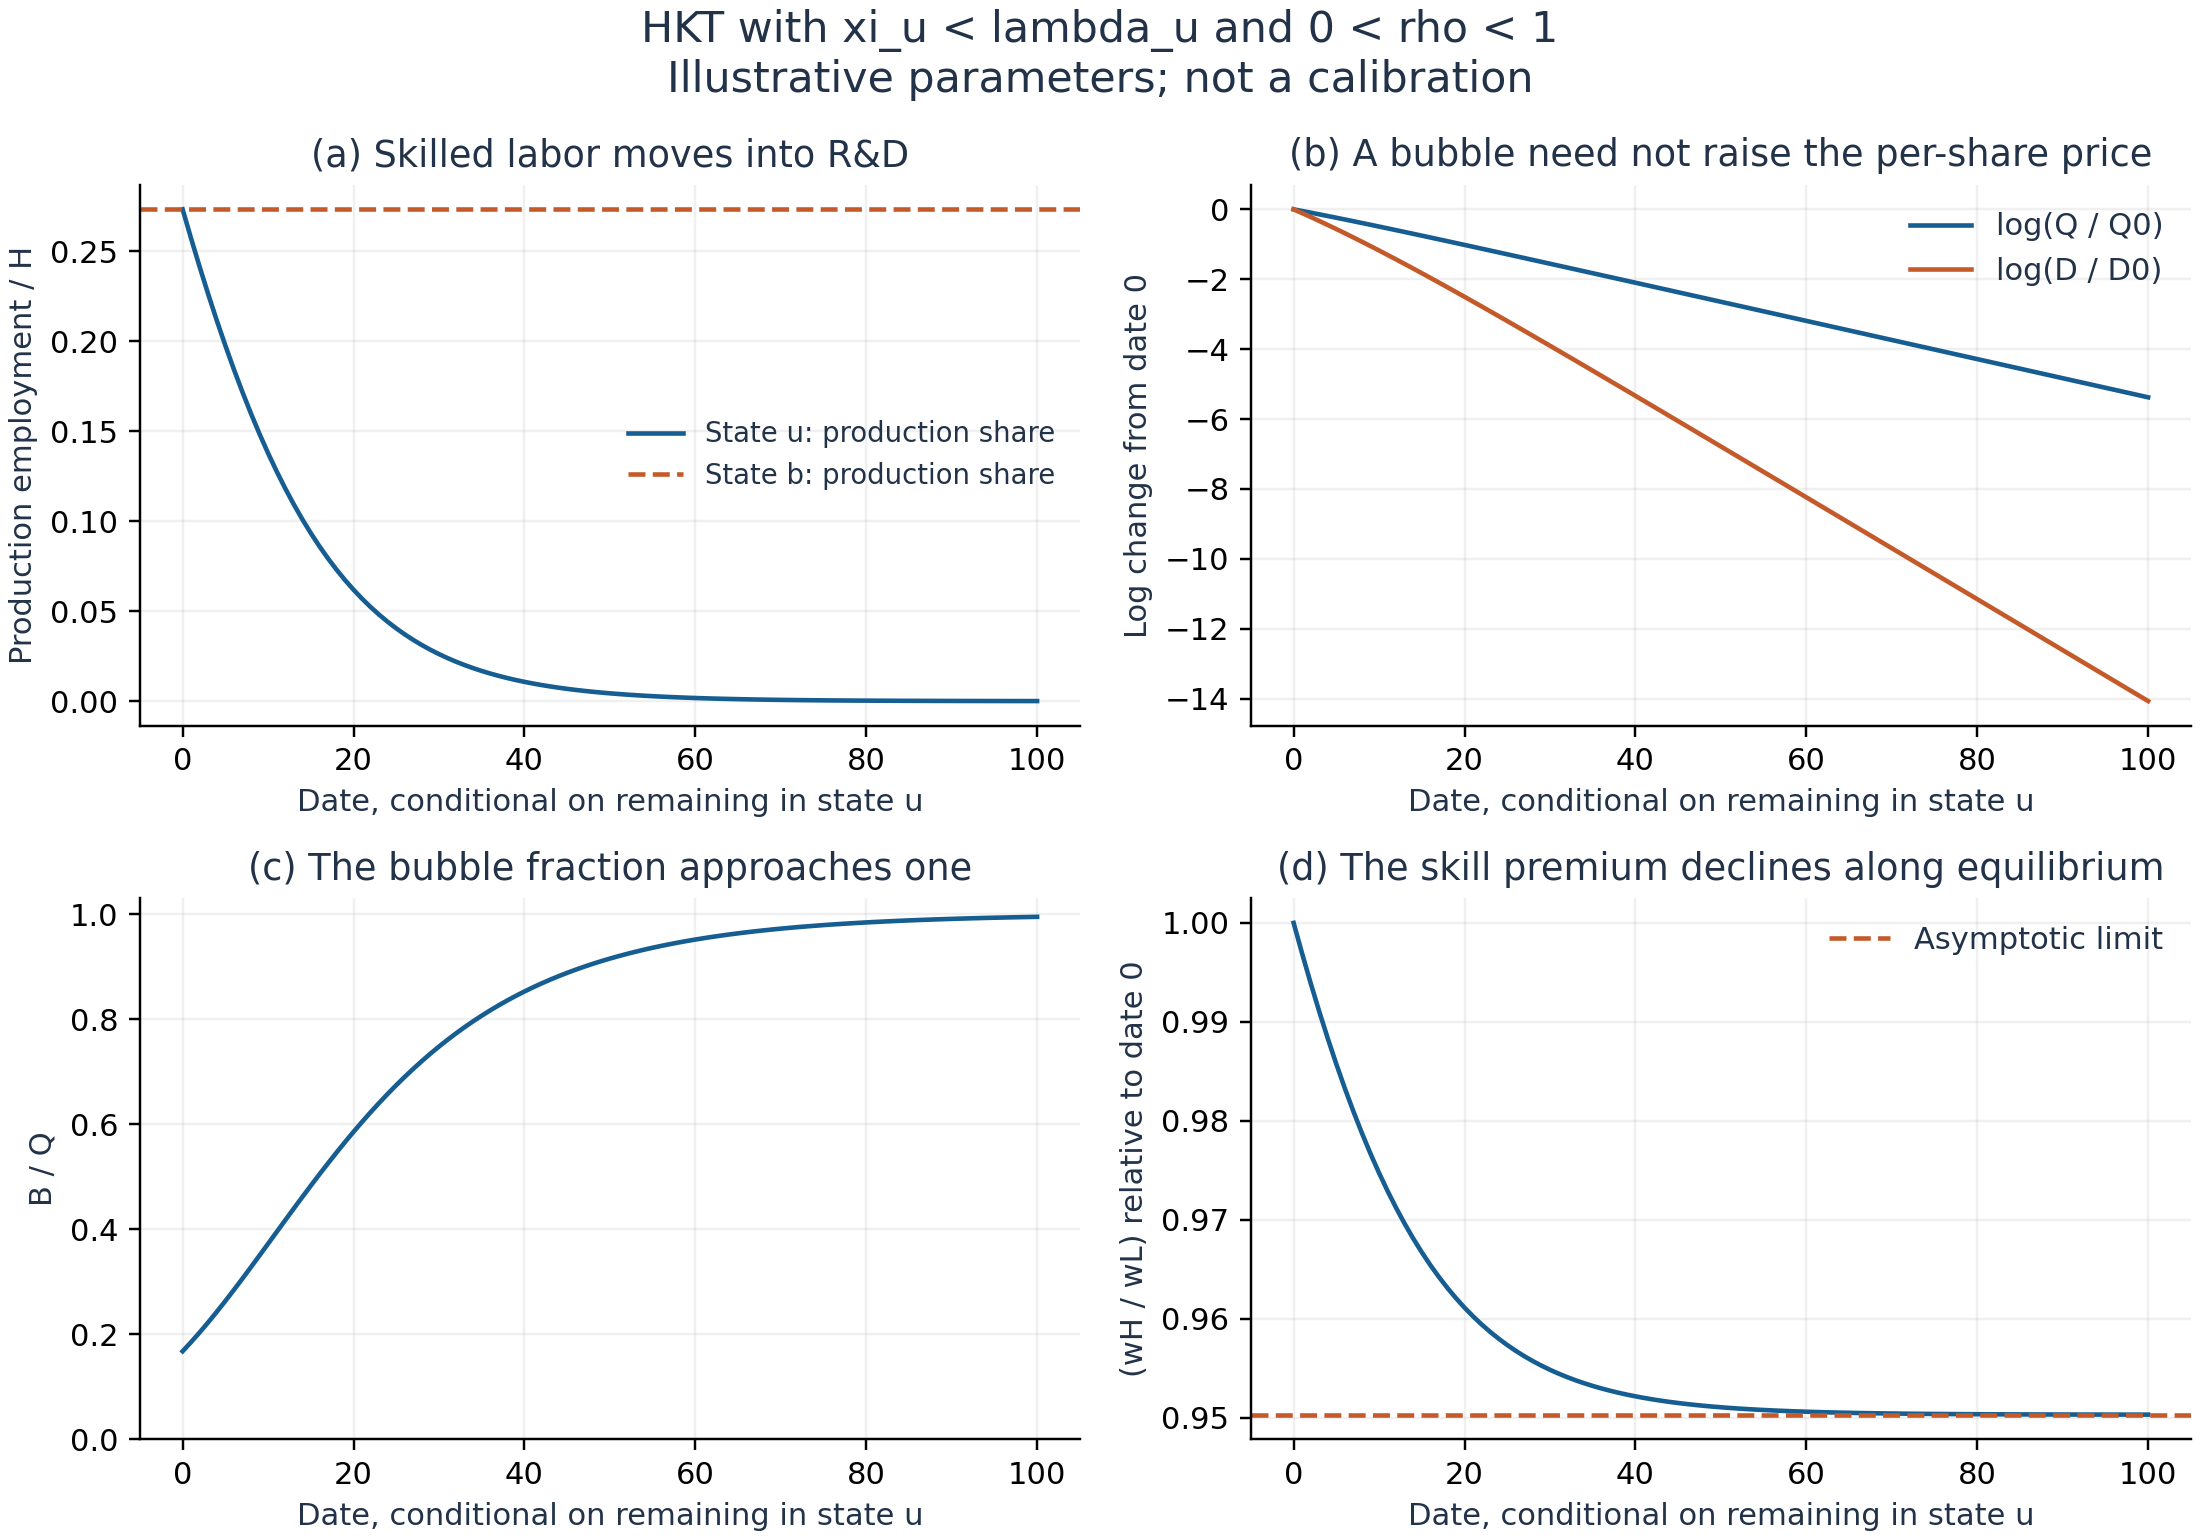
\includegraphics[width=\textwidth]{illustrative_paths.png}
\caption{Conditional state-$u$ dynamics. The balanced-state production share
in panel (a) is shown as a reference, not as a realized switch. In panel (c),
the finite-product truncation error is controlled by the bound above.}
\end{figure}

\begin{table}[htbp]
\centering\small
\caption{Correspondence with the user-supplied HKT paper.}
\begin{tabularx}{\textwidth}{@{}l l X@{}}
\toprule
HKT location & Printed pages & Use in this note\\
\midrule
(2.1), (2.4), Theorem 1 & 7--14 & Preferences, SDF, two-series bubble test\\
(3.2), (3.12)--(3.19) & 16--20 & CES production, dividends, occupation, share timing\\
Proposition 3.1, (3.23) & 20--21 & Unique equilibrium and the no-entry stock-price branch\\
Assumption 6, (4.1)--(4.4) & 21--23 & Spillovers, $\kappa>0$, initial innovation\\
Proposition 4.1, Theorem 2 & 23--25 & Knowledge growth and bubble necessity\\
Propositions 4.2--4.3 & 28--29 & IPO experiment and regime transition\\
Proposition 4.4 & 30--31 & Balanced-growth restrictions\\
Appendices A.4--A.8 & 37--42 & Growth, pricing, and comparative-static proofs\\
Theorem 3, Appendix B.1 & 32--33, 47--51 & Infinitely lived cohorts\\
Appendix B.2 & 52--59 & Scope of the non-unit-EIS extension\\
\bottomrule
\end{tabularx}
\end{table}

\end{document}
